\section{The Electronic Basis for Memory}

In our studies of computer science at the University of Alberta, we rarely mention the underlying electronics that form the basis of electronic logic systems, and hence computers. Despite our high level abstractions away from silicon when learning how to write code, a robust understanding of the underlying principles of computing systems encourages students to think about the physical limitations of our current systems and why we design our systems as we do. This section will scratch the surface of electrical engineering and provide the reader with the essential background to determine why certain artifacts, like CAS latency, appear in the analysis of the memory subsystem.

\subsection{The Transistor and Capacitor}

When studying memory systems, there are two fundamental structures we need to understand: the transistor and the capacitor. For our purposes it suffices to think of the capacitor as a battery and the transistor as a switch, the following section is an elaboration on those simplifications.

\begin{figure}
  \centering
  \begin{tikzpicture}
    % Draw the capacitor
    \draw (-2,1) -- (0,1) to[capacitor, l=$C$] (2,1) -- (4,1);
    
    % Add the image next to the capacitor
    \node at (3,-1) {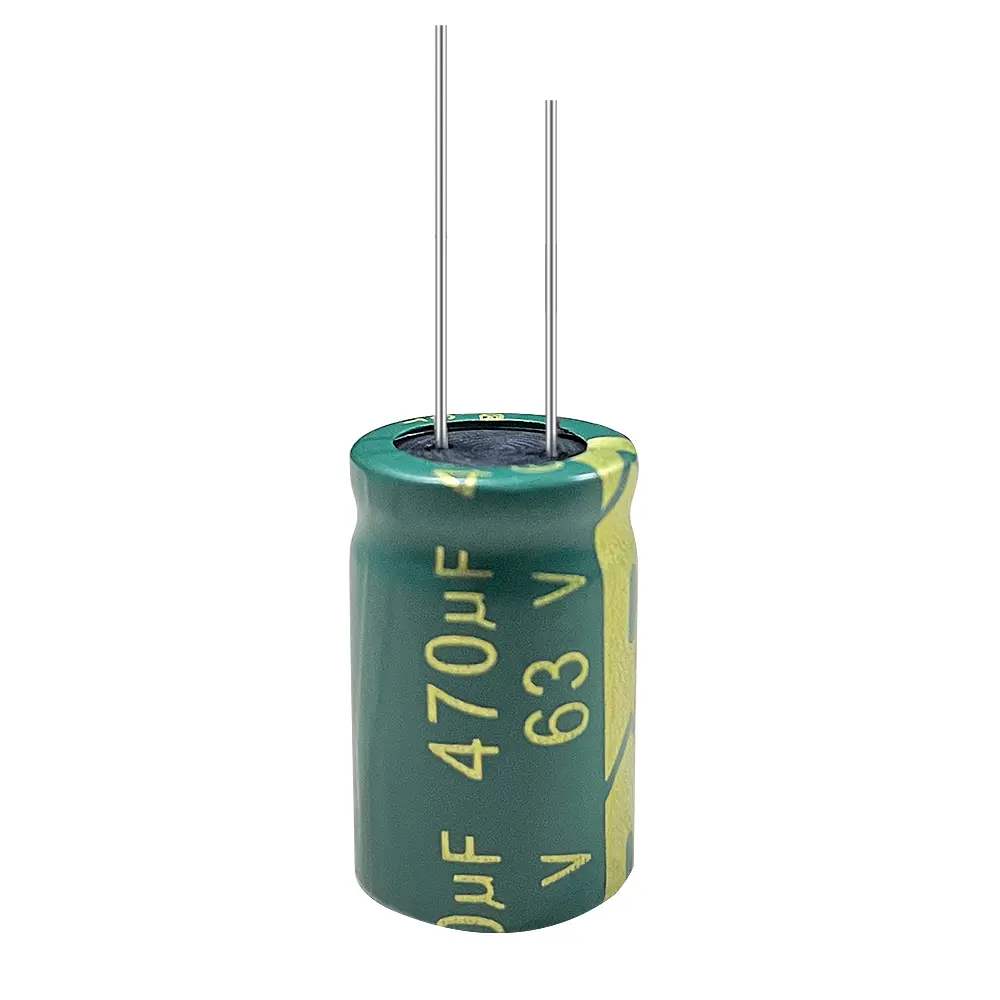
\includegraphics[width=2cm]{assets/capacitor.png}};
  \end{tikzpicture}
  \caption{A Capacitor.}
\end{figure}
Beginning with the capacitor, a capacitor accumulates and stores charge as the buildup of a potential difference between two surfaces insulated from each other CITE. They serve as the physical storage for a single bit in conjunction with a transistor and a ground. Charging a capacitor is a relatively slow operation (relative to the modification of an SRAM cell, as we will discuss in a moment), but the die area of a capacitor and single transistor is significantly less than the die area required for a single cell of SRAM, thus allowing us to produce large capacity DRAM cheaply CITE.

\begin{figure}
  \centering
  \begin{tikzpicture}
    % Draw the NMOS transistor
    \draw (0,0) node[nmos, anchor=D] (transistor) {};

    % Connect and label the source
    \draw (transistor.S) -- ++(0,-1) node[below] {Source};

    % Connect and label the drain
    \draw (transistor.D) -- ++(0,1) node[above] {Drain};

    % Connect and label the gate
    \draw (transistor.G) -- ++(-1,0) node[left] {Gate};

    % Add the image next to the transistor
    \node at (3,0) {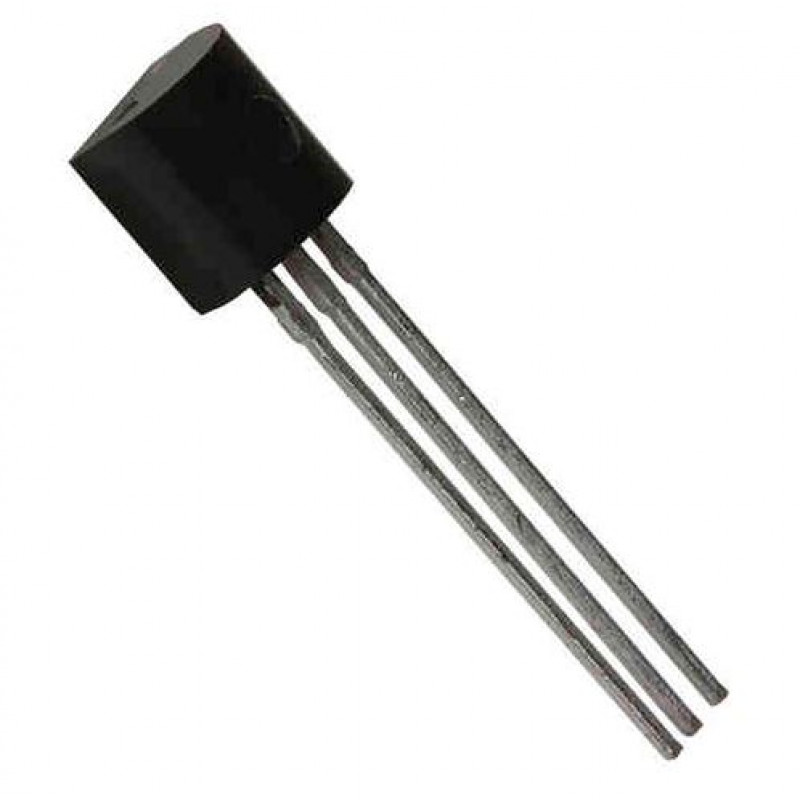
\includegraphics[width=2cm]{assets/transistor.jpg}};
  \end{tikzpicture}
  \caption{A Transistor.}
\end{figure}

The transistor is our next target of study. Simplistically, the transistor is a switch. It consists of three connections: the source, the gate and the drain. The gate serves as the switching mechanism: when we apply current to the gate, current can flow freely between the source and the drain. When no current is applied to the gate, no electricity can flow from the source and drain. The transistors used in hobby projects are often designed to be one-way transistors, however the transistors used in common DRAM systems are designed to allow current to flow both in and out with the same resistance CITE. Current transistor technology relies on the MOSFET paradigm, though Intel's upcoming \SI{16}{\angstrom} process is rumored to use RibbonFET/FINFET technologies CITE.

The transistor and capacitor form the basis for our current memory technologies.

\subsection{Storing a Single Bit}

\begin{figure}
  \centering
  \begin{circuitikz}
    % Transistor
    \draw (0,0) node[nmos, rotate=-90, anchor=S] (transistor) {};
    
    % Bit line
    \draw (transistor.S) -- ++(0,-1) node[below] {Bit Line};
    
    % Word line
    \draw (transistor.G) -- ++(-1,0) node[left] {Word Line};
    
    % Capacitor at the drain
    \draw (transistor.D) -- ++(1,0) to[capacitor] ++(0,-1) node[ground] {};
    
    % Label the drain-capacitor connection
    \node at ($(transistor.D) + (0.5,-0.3)$) {C};
  \end{circuitikz}
  \caption{A single DRAM cell.}
  \label{fig:dram-cell}
\end{figure}

We can combine the transistor and the capacitor to form a single DRAM cell as illustrated in figure~\ref{fig:dram-cell}. This unit allows us to store a single bit through the following process:
\begin{enumerate}
  \item Apply current to the bit line
  \item Apply current to the gate, resulting in a potential difference letting the capacitor charge
  \item Eliminating power to the gate, effectively locking the power into the capacitor
\end{enumerate}
A capacitor of this size loses its charge quickly, resulting in the need for periodic refresh of the entire DRAM array. This refresh essentially consists of reading and rewriting all of the elements in the array in order to maintain their charge.

\begin{figure}
  \centering
  \begin{tikzpicture}
  %FIXME
    % Parameters for layout
    \def\nrows{4} % Number of word lines
    \def\ncols{3} % Number of bit lines
    \def\cellwidth{2} % Width between columns
    \def\cellheight{2} % Height between rows

    % Draw word lines (horizontal lines)
    \foreach \y in {1,...,\nrows} {
        \draw[thick] (0, -\y*\cellheight) -- (\ncols*\cellwidth, -\y*\cellheight) node[right] {Word Line \y};
    }

    % Draw bit lines (vertical lines)
    \foreach \x in {1,...,\ncols} {
        \draw[thick] (\x*\cellwidth, 0) -- (\x*\cellwidth, -\nrows*\cellheight) node[below] {Bit Line \x};
    }

    % Draw DRAM cells (transistor and capacitor at each intersection)
    \foreach \x in {1,...,\ncols} {
        \foreach \y in {1,...,\nrows} {
            % Transistor
            \draw[nmos, rotate=-90, scale=0.5] (\x*\cellwidth-0.5, -\y*\cellheight) node (t\x\y) {};
            % Capacitor
            \draw (t\x\y.D) -- ++(0.5,0) to[capacitor] ++(0,-0.5) node[ground] {};
        }
    }
  \end{tikzpicture}
  \caption{A DRAM Array.}
  \label{fig:dram-array}
\end{figure}
We can chain the individual bit storage mechanisms together to form word lines and group those together to form the full DRAM array as shown in figure~\ref{fig:dram-array}. 
